\section{Background}
\label{sec:jol}
\label{sec:bg}

The Overlog language is sketched in a variety of papers.  Originally
presented as an event-driven language~\cite{p2}, it has evolved a semantics more carefully grounded in Datalog, the standard deductive
query language from database theory~\cite{ullmanbook}.  Our Overlog is
based on the description by Condie et al.~\cite{evitaraced}.  We briefly 
review Datalog here, and the extensions presented by Overlog.
%%We
%%review Datalog in Appendix~\ref{app:datalog}, and the extensions
%%offered by Overlog here.

The Datalog language is defined over relational tables; it is a purely logical query language that makes no changes to the stored tables. A Datalog \emph{program} is a set of \emph{rules} or named queries, in the spirit of SQL's \emph{views}.  A Datalog rule has the form:
\[
	r_{\mbox{\em head}}(\langle\mbox{\em col-list}\rangle) \mbox{{ \tt :- }} r_1(\langle\mbox{{\em col-list}}\rangle), \ldots, r_n(\langle\mbox{{\em col-list}}\rangle)
\]
Each term $r_i$ represents a relation, either \emph{stored} (a database table)
or \emph{derived} (the result of other rules).  Relations' columns are listed as
a comma-separated list of variable names; by convention, variables begin with
capital letters.  Terms to the right of the \texttt{:-} symbol form the rule
\emph{body} (corresponding to the {\tt \small FROM} and {\tt \small WHERE}
clauses in SQL), the relation to the left is called the \emph{head}
(corresponding to the {\tt \small SELECT} clause in SQL).  Each rule is a
logical assertion that the head relation contains those tuples that can be
generated from the body relations.  Tables in the body are joined together based
on the positions of the repeated variables in the column lists of the body
terms.  For example, a canonical Datalog program for recursively computing all
paths from links~\cite{loo-sigmod06} is shown in Figure~\ref{fig:datalogsql}
(ignoring the Overlog-specific {\tt @} notation), along with an SQL translation.
Note how the SQL {\tt \small WHERE} clause corresponds to the repeated use of
the variable {\tt \small To} in the Datalog.

%\rcs{START} Overlog extends Datalog with distribution and a semantics for table updates.
%\rcs{END Between START, END isn't really true in \JOL, and is (I
%think) a confusing way to think about location specifiers.  For one
%thing, \JOL doesn't partition the tables, because it doesn't
%understand membership.  Also, \JOL supports local tables, and
%networks that contain multiple programs.  Recommend next paragraph
%instead.}
\begin{figure}[t]
%\begin{minipage}{0.5\linewidth}
\begin{footnotesize}
\begin{verbatim}
path(@From, To, To, Cost) 
        :- link(@From, To, Cost);
path(@From, End, To, Cost1 + Cost2)
        :- link(@From, To, Cost1),
           path(@To, End, NextHop, Cost2);
\end{verbatim}
\end{footnotesize}
%\end{minipage}
%\begin{minipage}{0.5\linewidth}
\begin{footnotesize}
\begin{verbatim}
WITH RECURSIVE path(Start, End, NextHop, Cost) AS
(   SELECT From, To, To, Cost FROM link
    UNION
    SELECT link.From, path.End, link.To,
           link.Cost + path.Cost
      FROM link, path
     WHERE link.To = path.Start );
\end{verbatim}
\end{footnotesize}
%\end{minipage}
\vspace{-8pt}
\caption{Example Overlog for computing all paths from links, along with an SQL translation.}
\label{fig:datalogsql}
\end{figure}


Overlog extends Datalog in three main ways: it adds notation to
specify the location of data, provides some SQL-style extensions such
as primary keys and aggregation, and defines a model for processing
and generating changes to tables.  Overlog supports relational tables
that may optionally be ``horizontally'' partitioned row-wise across a
set of machines based on a column called the \emph{location specifier},
which is denoted by the symbol {\tt @}.
%A tuple is stored at the address specified in its location specifier column.
%  \JOL generalizes this slightly by supporting ``local'' tables that have no location specifier.  This is a notational shorthand to prevent bugs: the same effect can be achieved by adding an additional location specifier column such tables, and ensuring that the value for each tuple is always ``localhost''.
%\rcs{Killed footnote; still object to saying tables are ``horizontally partitioned''.  It would be crisper/more accurate to say this:  Overlog rules contain {\em location specifiers} which are denoted by the symbol {\tt @}.  Each tuple is stored at the address specified in its location specifier column.  OPTIONALLY:  A join against a location specifier column produces a list of machines that should be involved in a rule's evaluation; a more complete discussion of rule localization is available in \cite{sigmod06xxx}}.  A subset of columns may be marked as the table's primary key, in which case no two rows may match on those columns.  By default, the primary key consists of all columns, implying that no two rows of a table may be identical.
% 
% A \JOL  network may be partitioned into sub-networks with ``private'' versions of the same table and library, or even contain different schemas and programs.  This allows us to compose \JOL services and simplifies Overlog programs that must reason about network partitioning, nodes with inconsistent data, and explicit state transfer.  
% 
%\rcs{move next sentence before primary key discussion?}
%%(Appendix~\ref{app:datalog} shows a standard network routing example from previous papers on declarative
%%networking.)
%\rcs{ cut rest of paragraph?}A location specifier column contain legal network addresses. 
% \rcs{<- This sentence isn't true: loc specifiers are ``String'' typed: if the schema knew about location specifiers, some programs would be harder to express.}  
%\JOL supports an extensible set of network address types, but we focus on IP address:port pairs in this paper.
 % corresponding to different protocols, though for this paper we implemented TCP and UDP, and hence location specifiers are on IP address:port pairs.  

%\jmh{Add a little on partitioning inducing communication, and cite SIGMOD '06 for localization.  Point out that the SQL is single-site, but the Overlog is part of a functioning routing protocol implementation.} \rcs{Does my redefinition of location specifier handle this?}

\begin{figure}[t]
  \centering
    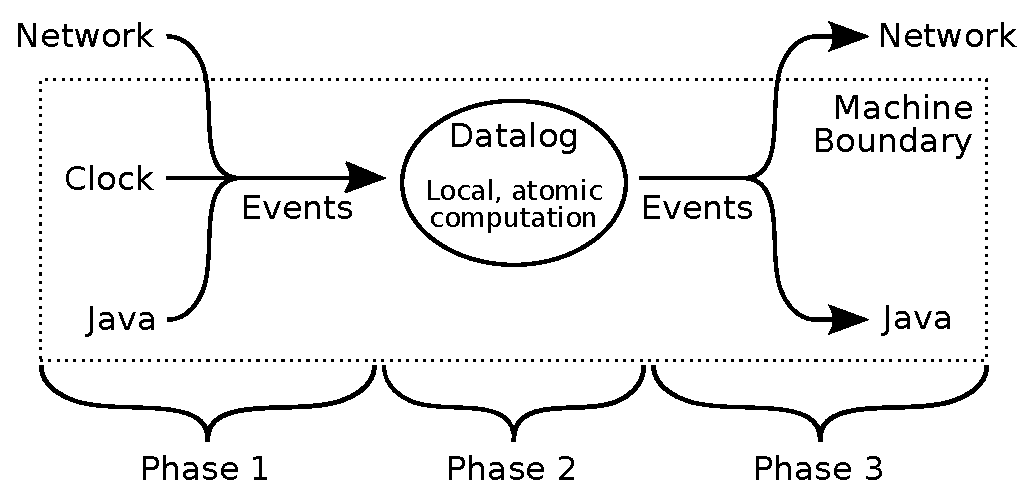
\includegraphics[width=0.95\linewidth]{jol-node.pdf}
    \label{fig:jol-node}
    \caption{An Overlog timestep at a participating node: incoming
      events are applied to local state, the local Datalog program 
      is run to fixpoint, and outgoing events are emitted.}
\vspace{-8pt}
\end{figure}

When Overlog tuples arrive at a node either through rule evaluation or
external events, they are handled in an atomic local Datalog
``timestep.'' Within a timestep, each node sees only locally-stored
tuples.  Communication between Datalog and the rest of the system
(Java code, networks, and clocks) is modeled using \emph{events}
corresponding to insertions or deletions of tuples in Datalog tables.

Each timestep consists of three phases, as shown in Figure~\ref{fig:jol-node}.
In the first phase, inbound events are converted into tuple insertions and
deletions on the local table partitions.  The second phase interprets the local rules and tuples according to traditional Datalog semantics, executing the rules to a ``fixpoint'' in a traditional bottom-up fashion~\cite{ullmanbook},
recursively evaluating the rules until no new results are generated.  In the
third phase, updates to local state are atomically made durable, and outbound
events (network messages, Java callback invocations) are emitted. Note that
while Datalog is defined over a static database, the first and third phases allow
Overlog programs to mutate state over time.

% Communication in Overlog happens as a side-effect of data partitioning. Loo et al.\ show that any Overlog program can be compiled into 
% a form where the body relations join on the same location-specifier variable, so that all relational processing is localized~\cite{loo-sigmod06}.  They also prove eventual consistency of the distributed tables under the rules, when certain simplifying assumptions hold.  In Section~\ref{sec:lessons} we discuss our experience with this model.

%\rcs{Rewrote this; the old discussion doesn't match the current implementation; the difference between the two is important for atomicity + transactions.  OLD: Each timestep consists of five phases.
% , which taken together atomically modify a local database, execute a Datalog program on that database, materialize the consequences of the program, and generate messages.  
%In Phase 1 ({\em Insertion}), inbound tuples are dequeued from a {\em network insertion queue}; each tuple arrives annotated with the name of a table, into which it is inserted\footnote{Tuples that do not conform to the local database schema are inserted into an ``exception'' table that can be configured either to store or drop tuples. \jmh{Is this a lie?}}.  In Phase 2 ({\em Datalog}), the Overlog rules in the system are treated as purely declarative Datalog queries, which are run recursively to their conclusion: a fixpoint where further application of the rules produces no new results. \JOL uses a delta-computation approach to speed up this process~\cite{matview-maintain}. In Phase 3 ({\em Materialization}), the outputs of Phase 2 queries that have the local address in their location specifier are cached in the local database as {\em Materialized Views}~\cite{matview-maintain}; output tuples with remote location specifiers are enqueued to be sent to their appropriate destination.
%Overlog supports syntax for tuple deletion and update as well, as described by Condie~\cite{evitaraced}.  
%  The exception to this processing are the results of Overlog rules prefaced by the {\tt delete} keyword; local {\tt delete} results are enqueued for Phase 4, whereas remote {\tt delete} results are marked as {\tt deletion} tuples before they are enqueued on the network.  \jmh{skipping primary key stuff here; roll in later if needed.} 
%In Phase 4 ({\em Deletion}), tuples are dequeued from an inbound {\em network deletion queue} and combined with the results of deletion tuples derived in Phase 2; taken together, these tuples are processed via deduction to determine any {\em consequent} tuples (previously computed in Phases 2 and 3 at any timestep) that  depend upon them recursively; then the tuples to be deleted {\em and all their local consequents} are deleted from the database; remote deletion consequents are also added to the network queue.  Finally, in Phase 5 ({\em Transmission}) the outbound network queues are flushed using the appropriate network protocols.}

\subsection{JOL}
The original Overlog implementation (\emph{P2}) is aging and targeted at network
protocols, so we developed a new Java-based Overlog runtime we call \emph{\JOL.}
Like P2, \JOL compiles Overlog programs into pipelined dataflow graphs of
operators (similar to ``elements'' in the Click modular router~\cite{click}).
\JOL provides \emph{metaprogramming} support akin to P2's Evita Raced
extension~\cite{evitaraced}: each Overlog program is compiled into a
representation that is captured in rows of tables.  Program testing,
optimization and rewriting can be written concisely as metaprograms in Overlog
that manipulate those tables.

Because the Hadoop stack is implemented in Java, we anticipated the need for
tight integration between Overlog and Java code. Hence, \JOL supports Java-based
extensibility in the model of Postgres~\cite{postgres}.  It supports Java
classes as abstract data types, allowing Java objects to be stored in fields of
tuples, and Java methods to be invoked on those fields from Overlog.  \JOL also
allows Java-based aggregation functions to run on sets of column values, and
supports Java \emph{table functions}: Java iterators producing tuples, which can
be referenced in Overlog rules as ordinary relations. We made significant use of
each of these features in \BOOMA.

  % \rcs{<- too dense; sounds complicated.  replace w/ figure that describes syntax?}  
% Second, \JOL makes use of Java's built-in networking code rather than implementing it as componentized dataflow as in P2.\rcs{<- implementation detail (cut)?}  
% Third, 
%\jmh{Removed discussion of metaprogrammed scheduler since we don't exercise it much.}
%In addition, inspired by the ideas of Evita Raced, we metaprogrammed \JOL's core execution loop and scheduler in Overlog as well.  Rather than using a traditional event loop,  in \JOL all inbound events (i.e., tuples) are passed into a single dataflow compiled from the system's runtime metaprogram. This dataflow ``routes'' tuples to appropriate branches corresponding to different rules, using a scheduler specified in Overlog.  Space prevents a thorough discussion of this design, but we mention it here because of our experience modifying the runtime rules as described in Section~\ref{sec:perf}.  
% \rcs{Fourth, \JOL's design is based upon composition of local datalog processes; P2's execution model attempted to provide coherent datalog semantics across network links.  We believe that \JOL's model leads to more natural handling of issues such as node failure and hetergeneous networks.}

%Our commercial cluster experiments ran on 96 physical nodes spanning 5 racks. Each node has 4 disks, 3 GB of memory, and 8 Intel Xeon processors\rcs{``Intel Xeon'' means nothing... are they 64 bit? Penitum IV generation? Core 2?}, 1.8 GHz each. One node was running the JobTracker, another node was running HDFS's NameNode. The other 94 nodes in the cluster were slaves running both a TaskTracker and a DataNode.

%\jmh{add details ...} \rcs{good enough?}
